% !TEX program = xelatex
\documentclass[11pt,a4paper]{article}

\usepackage[margin=2.2cm,headheight=14pt]{geometry}
\usepackage{fontspec}
\usepackage{xeCJK}
\xeCJKsetup{AutoFakeBold=true}
\setmainfont{Times New Roman}
\setCJKmainfont{STKaiti}
\setmonofont{Menlo}[Scale=0.85]
\setCJKmonofont{STKaiti}
\usepackage{amssymb}
\usepackage{booktabs}
\usepackage{tabularx}
\usepackage{array}
\usepackage[table]{xcolor}
\usepackage{enumitem}
\usepackage{fancyhdr}
\usepackage[most]{tcolorbox}
\usepackage{tikz}
\usetikzlibrary{arrows.meta}
\usepackage[hidelinks]{hyperref}
\usepackage{xurl}
\urlstyle{same}

\setlength{\parindent}{0pt}
\setlength{\parskip}{4pt}
\setlength{\emergencystretch}{2em}
\setlist{itemsep=3pt,topsep=3pt}
\renewcommand{\arraystretch}{1.2}

\pagestyle{fancy}
\fancyhf{}
\fancyhead[L]{AI-in-the-Loop in Software Project Cycle}
\fancyhead[R]{Group 07 --- CP1}
\fancyfoot[C]{\thepage}

\definecolor{codebg}{RGB}{242,241,236}
\definecolor{codecm}{RGB}{110,110,110}

\newtcolorbox{keybox}{breakable,colback=codebg,colframe=codecm,boxrule=0.4pt,arc=1pt,
  left=4pt,right=4pt,top=2pt,bottom=2pt}

\newcommand{\q}[1]{``\emph{#1}''}
\newcommand{\code}[1]{\texttt{#1}}
\newcommand{\ra}{$\rightarrow$}
\newcolumntype{L}{>{\raggedright\arraybackslash}X}

\begin{document}

\begin{center}
  {\LARGE\bfseries Checkpoint 1 (CP1)}\\[2pt]
  {\large DecisionTrace: AI-assisted decision memory for student software teams}
\end{center}

\begin{tabular}{@{}ll}
  \textbf{Course:} & CSIC30216 AI-in-the-Loop in Software Project Cycle, Fall 2026 \\
  \textbf{Team number:} & Group 07 \\
  \textbf{Members:} & 周廷威 (112550013), 林彥宇 (112550098), \\
  & 蔡凱旭 (112550153), 蔡尚融 (112550201) \\
  \textbf{Repository:} & \url{https://github.com/Apollo58168/NYCU_AI-in-the-Loop-in-Software-Project-Cycle} \\
  \textbf{Date:} & 25 October 2026 \\
\end{tabular}

%==========================================================
\section{Team Charter}
%==========================================================

\subsection{How we make decisions when we disagree}\label{sec:disagree}

\begin{enumerate}
  \item \textbf{Raise it in writing.} Whoever disagrees opens a thread in our Discord \code{\#decisions} channel (or comments on the GitHub PR/issue), stating the options and the argument for each in a few sentences.
  \item \textbf{Evidence first, 48-hour window.} For 48 hours after the thread is opened, each side may add evidence: a test, a prototype, documentation, user feedback, or a course requirement. Following our \code{AI\_GUIDELINES.md}, correctness and safety questions are settled by evidence (tests, specs, docs), never by vote; if the evidence does not settle them, the code steward decides after hearing both sides. Style questions are settled by the formatter/linter and documented conventions. Steps 3--4 apply only to scope and preference questions.
  \item \textbf{Decide once the window has closed.}
  \begin{itemize}
    \item \emph{Non-blocking} questions are decided at the \textbf{first weekly sync after the window closes}. A thread opened less than 48 hours before a sync therefore waits for the following sync.
    \item \emph{Blocking} questions (someone cannot continue their task) are decided in the thread \textbf{as soon as the window closes}, or earlier if all four agree.
  \end{itemize}
  If all four agree, we are done. Otherwise we take a \textbf{majority vote (3 of 4)}: by voice at the sync, or, for blocking questions, by a Discord poll that stays open for 24 hours.
  \item \textbf{Tie or still stuck} (2--2, or no option reaches 3 votes when the poll closes): the \textbf{owner of the affected work} decides scope/product questions, and the \textbf{current code steward (林彥宇, GitHub \code{Apollo58168})} decides anything that touches \code{main} (architecture, merge decisions). The decider must hear both positions first.
  \item \textbf{Record it.} If the decision is made in a PR, it is recorded in that PR (see the definition of done). Otherwise, within 48 hours of the decision, the person who opened the thread adds any significant decision (architecture, data model, evaluation method, scope) to \code{DECISIONS.md} through a PR, with \emph{What / Why / Alternative rejected / Led by}. A recorded decision is reopened only if new evidence appears, not because someone missed the discussion.
\end{enumerate}

\subsection{Definition of done}

A piece of work is \textbf{done} only when someone else can check every box below:

\begin{itemize}[label=$\square$]
  \item The work is on a branch and merged into \code{main} through a \textbf{pull request} (no direct pushes; the branch ruleset in \S\ref{sec:repo} enforces this).
  \item The PR description follows \code{.github/PULL\_REQUEST\_TEMPLATE.md}, including the \emph{Decision} section when a significant choice was made.
  \item \textbf{At least one teammate other than the author approved} the PR (also enforced by the ruleset), and that reviewer can explain what the change does.
  \item For code: it runs locally, and relevant tests exist and pass. For AI-drafted tests, a human checked that they can fail.
  \item If AI produced retained code or text, the PR says so and links a \code{PROMPT\_LOG.md} entry.
  \item If a significant choice was made, \code{DECISIONS.md} is updated in the same PR.
  \item The linked GitHub issue (if any) is closed.
\end{itemize}

\subsection{Communication outside class}

\begin{tabularx}{\linewidth}{@{}>{\bfseries}p{2.6cm}L@{}}
\toprule
What & Agreement\\
\midrule
Channel & \textbf{Discord} team server: \code{\#general} for coordination, \code{\#decisions} for disagreements and decisions, \code{\#pr-review} for review requests. GitHub PR/issue comments for anything tied to code.\\
Frequency & One \textbf{weekly 30-minute Discord voice sync} (time fixed at the start of each week, default Sunday evening), plus short async progress updates in \code{\#general} at least twice a week.\\
Response time & Reply to a direct mention within \textbf{24 hours} (within \textbf{12 hours} in the 3 days before a deadline). Pick up PR review requests within \textbf{48 hours}. Announce any absence longer than 2 days in \code{\#general} in advance.\\
Escalation & If someone has not responded after 48 hours, the code steward reassigns the blocking task and notes it at the next sync.\\
\bottomrule
\end{tabularx}

%==========================================================
\section{Problem Statement with Evidence}\label{sec:problem}
%==========================================================

\subsection{The problem}

\begin{keybox}
In multi-week student software teams (for example, teams that use GitHub with Discord or LINE), members often need to know \emph{why} an earlier technical choice was made: they joined late, took over a teammate's module, or are reviewing a PR that touches older code. The reasoning is scattered across chat threads, PR comments, meeting notes and people's memories. So they either interrupt the one teammate who remembers or guess. The consequences we are investigating are \textbf{reopened debates, rework, and deliberate choices being reverted by mistake}.
\end{keybox}

\textbf{Who experiences it:}
\begin{itemize}
  \item \textbf{Late joiners / module inheritors}: students who take over work mid-semester (a teammate dropped, or tasks were rebalanced).
  \item \textbf{The ``team memory'' person}: usually the team lead or repo maintainer, who is repeatedly interrupted with ``why did we do X?''.
  \item \textbf{PR reviewers}: who must judge a change without knowing the constraints behind the code it touches. [H] Not yet interviewed (\S\ref{sec:evidence}).
\end{itemize}

\textbf{What it is \emph{not}:} general team communication or meeting scheduling. The scope is narrowly \emph{recovering the reason behind a technical decision that has already been made}.

\textbf{Internal observation [I] (our own repo, not user evidence):} four of our five merged PRs (\#1, \#3--\#5) were onboarding tests that added a name to \code{CONTRIBUTORS.md}. The one substantive PR, \#6, set our Week~3 evaluation method, but no \code{DECISIONS.md} entry records that choice or its reasons. This is one data point from the team proposing the tool, so we use it only as an illustration.

\subsection{Evidence from users}\label{sec:evidence}

\textbf{Evidence labels used in this report.} \textbf{[R]} real interview with a person outside our team; \textbf{[I]} internal observation of our own repository; \textbf{[H]} design hypothesis still to be tested. Only [R] counts as evidence from real users.

\subsubsection*{Real-user interviews [R]}

Two 15-minute Google Meet interviews on 23 October 2026 with people outside our team, recruited through personal contacts and anonymized as R1 and R2; both agreed to be cited anonymously. Their points are reported in our own words from the interviewers' notes. The ``On the tool'' points are reactions to our idea, described in question~7 of the guide (Appendix~A).

\paragraph{R1 --- late joiner.}
\emph{4th-year Electrical Engineering undergraduate. Interviewed by 蔡凱旭.}
\begin{itemize}
  \item \textbf{Incident:} found timestamps stored as \code{TEXT} instead of \code{timestamptz} and assumed it was a mistake, but wanted to check before changing it. A Discord search for ``timestamp''/``timezone'' gave $\sim$60 hits, mostly noise. The schema PR had been squash-merged as ``init db'', and the HackMD notes stopped at week 5. It took $\sim$1.5 hours, and they found only half an answer: the decision had been made in a voice call.
  \item \textbf{Asking the author:} got a next-day reply in which the author was unsure, only guessing that the frontend date library had caused problems. R1 reported that even the person who made the decision did not fully remember, and it felt awkward to question the work as the new member.
  \item \textbf{Cost:} wrote the migration anyway. It broke the frontend's date parsing and was reverted ($\sim$half a day, 2 people). The team also re-argued ``JWT vs.\ sessions'', which had been settled in week 4.
  \item \textbf{Coping today:} \code{git blame} \ra{} open the PR \ra{} search Discord around the PR's merge date. This sometimes works but is slow.
  \item \textbf{On the tool:} source links matter most. R1 was skeptical that AI might turn a mundane explanation into a smarter-sounding but inaccurate one, which would be worse than having no explanation. Would approve 3--5 cards/week if it is one click in Discord, but would ignore a separate site like HackMD. Raised privacy concerns about venting in Discord and wants a \code{temporary / revisit later} flag.
\end{itemize}

\paragraph{R2 --- the ``team memory'' person.}
\emph{4th-year Computer Science undergraduate. Interviewed by 林彥宇.}
\begin{itemize}
  \item \textbf{Incident:} three weeks before the demo, a teammate asked why the app polled every 10\,s instead of using WebSockets. WebSockets kept dropping behind the school VM's reverse proxy, and the TA approved polling. R2 spent $\sim$20 min scrolling LINE for the proxy-error screenshot because the teammate did not believe the explanation without proof.
  \item \textbf{Frequency and cost:} 2--3 ``why'' questions per week, 2--20 min each (by our calculation, up to $\sim$1\,h/week). R2 said the time itself was not the main problem; the context switching was. They started a \code{DECISIONS.md} in week 3 with $\sim$5 entries; nobody else edited it, and it was abandoned by week 7. R2 found there was no clear moment to write an entry, because decisions settle gradually over about three days of chat. A teammate later switched image storage to base64 in the database, despite an earlier decision against it for size reasons. The database bloated and the change was reverted ($\sim$1 day, 2 people); the Provider-vs-Riverpod debate was reopened twice.
  \item \textbf{On the tool:} would give it $\sim$15 min/week, batched before the weekly meeting, not as all-day notifications. R2's biggest fear was a plausible but wrong reason that \emph{looks authoritative}. Would reject the tool if they ended up the only reviewer again, if it drafted $\sim$30 trivial cards a week, or if it needed a manual LINE export every time. R2 saw value in letting teammates ask the tool why a decision was made so they would stop interrupting R2.
\end{itemize}

\subsubsection*{What the evidence does and does not show}

Two interviews are exploratory, not a representative sample: they show that the problem occurred, and was costly, for these two people, not how common it is among student teams. Neither interviewee was asked directly whether our framing fits their experience; we will ask this in the weeks 8--9 interviews.

\textbf{Validation plan.} Neither R1 nor R2 covers the PR-reviewer role. In weeks 8--9, before building past a prototype, we will run the same guide with \textbf{at least 3 additional real students} (at least one PR reviewer, plus another late joiner and maintainer). Where they disagree with R1 and R2, we revise \S\ref{sec:problem}--\S\ref{sec:eval} and record the disagreement.

\subsection{Why existing tools and approaches do not solve it}\label{sec:existing}

{\small
\begin{tabularx}{\linewidth}{@{}>{\raggedright\arraybackslash}p{3.1cm}L>{\raggedright\arraybackslash}p{4.0cm}@{}}
\toprule
\textbf{Existing tool / approach} & \textbf{What it fails to do for \emph{this} problem} & \textbf{From interviews} (R1, R2 [R])\\
\midrule
\textbf{Discord / LINE search} & Keyword-only, so you must already know the word people used. Reasoning is spread over dozens of messages, and voice calls leave nothing. Nothing links a message to the code it is about. & R1: $\sim$60 noisy hits for ``timestamp''. R2: 20 min scrolling LINE for a screenshot.\\
\textbf{\code{git blame} + PR history} & Shows \emph{who} and \emph{when}, not \emph{why}. Squash merges and ``LGTM''/``fix'' descriptions drop the discussion, which usually happened in chat anyway. Breaks after file moves. & R1: schema PR titled ``init db''.\\
\textbf{Hand-written decision log / ADR} (\code{DECISIONS.md}) & The right \emph{format}, but nobody maintains it. Writing an entry is extra work, and decisions settle gradually, so there is no obvious moment to write one. Entries go stale and do not link to code. & R2's log died by week 7.\\
\textbf{Meeting notes} (HackMD / Notion) & Record \emph{what} and \emph{who does what}, rarely \emph{why}. Stop being updated mid-semester. Not linked to commits. & R1: notes stopped at week 5.\\
\textbf{Asking the teammate who remembers} & Works, but interrupts that person, depends on their memory, and fails once they have left. & R2: up to $\sim$1\,h/week, and the context switching mattered more. R1: the author was unsure.\\
\textbf{General AI chat} (e.g.\ pasting history into ChatGPT) & Can summarize, but produces no persistent, team-approved record, and may present a guessed reason as fact with no source link. & Our inference from R1's and R2's trust concerns, not a tool they reported using.\\
\bottomrule
\end{tabularx}
}

\textbf{The gap DecisionTrace targets:} each approach above fails at one of two points. Chat search, \code{git blame} and asking a teammate keep the reasoning but make it \emph{slow to recover}; decision logs and meeting notes make it quick to recover but \emph{nobody writes them}. DecisionTrace combines the \emph{low writing cost} of AI drafting with the \emph{trustworthiness} of a human-approved log, in which every reason links to its source and is marked \code{unknown} when the sources do not support it. Whether teams will actually keep doing the review step is the main open risk [H]; this evaluation measures review cost per card, not whether teams keep reviewing over a semester.

%==========================================================
\section{Initial Interaction Design Sketch}\label{sec:design}
%==========================================================

\subsection{What the tool does}

DecisionTrace turns the places where teams \emph{already} discuss decisions (PRs, issues, commits, chat threads, meeting notes) into a searchable, \textbf{human-approved decision log}. An AI drafts \textbf{decision cards} from those sources. A teammate approves, edits, or rejects each card, and approved cards are added to \code{DECISIONS.md} through a PR. Later, anyone can ask ``why did we choose X?'' and get the approved card, with links back to the original discussion.

\subsection{Inputs and outputs}

\textbf{Inputs}

{\small
\begin{tabularx}{\linewidth}{@{}>{\raggedright\arraybackslash}p{4.2cm}L@{}}
\toprule
\textbf{Input} & \textbf{Format (v1 unless marked \emph{later})}\\
\midrule
GitHub pull requests, issues, commits & Fetched for one repository via the GitHub REST API: title, description, review comments, linked issues, merge date, commit SHA.\\
Chat discussions & Plain text pasted by the author: only the messages of one thread, from an opted-in channel, that are about this decision (Discord or LINE). \emph{Later:} a Discord bot that reads opted-in threads directly.\\
Meeting notes & Markdown files exported from HackMD or Notion.\\
Question (retrieval mode) & Free text, e.g.\ ``Why did we choose PostgreSQL over MongoDB?''\\
\bottomrule
\end{tabularx}
}

\textbf{Outputs}
\begin{enumerate}
  \item \textbf{Decision card (candidate)}: structured JSON/Markdown with these fields:
  \begin{itemize}
    \item \code{decision}: the choice that appears to have been made
    \item \code{reason}: only reasons the sources state, each with the \textbf{verbatim quoted passage} it relies on; otherwise \code{unknown}
    \item \code{alternatives}: options explicitly considered in the sources
    \item \code{sources}: exact links (PR number, comment URL, commit SHA, note line, pasted-thread line)
    \item \code{confidence}: low / medium / high, with a one-line justification (a review signal, not proof)
    \item \code{status}: Pending \ra{} Approved / Edited / Rejected (also \code{temporary}, \code{superseded by \#\ldots}), with reviewer name and time
  \end{itemize}
  \item \textbf{Decision log}: approved and edited cards, appended to \code{DECISIONS.md} through an auto-opened PR, so they follow our normal review rules.
  \item \textbf{Answer to a question}: the matching approved card(s) with source links, or ``no approved decision found''. It never invents an answer from the raw history.
\end{enumerate}

\subsection{How two people interact with it}

\begin{center}
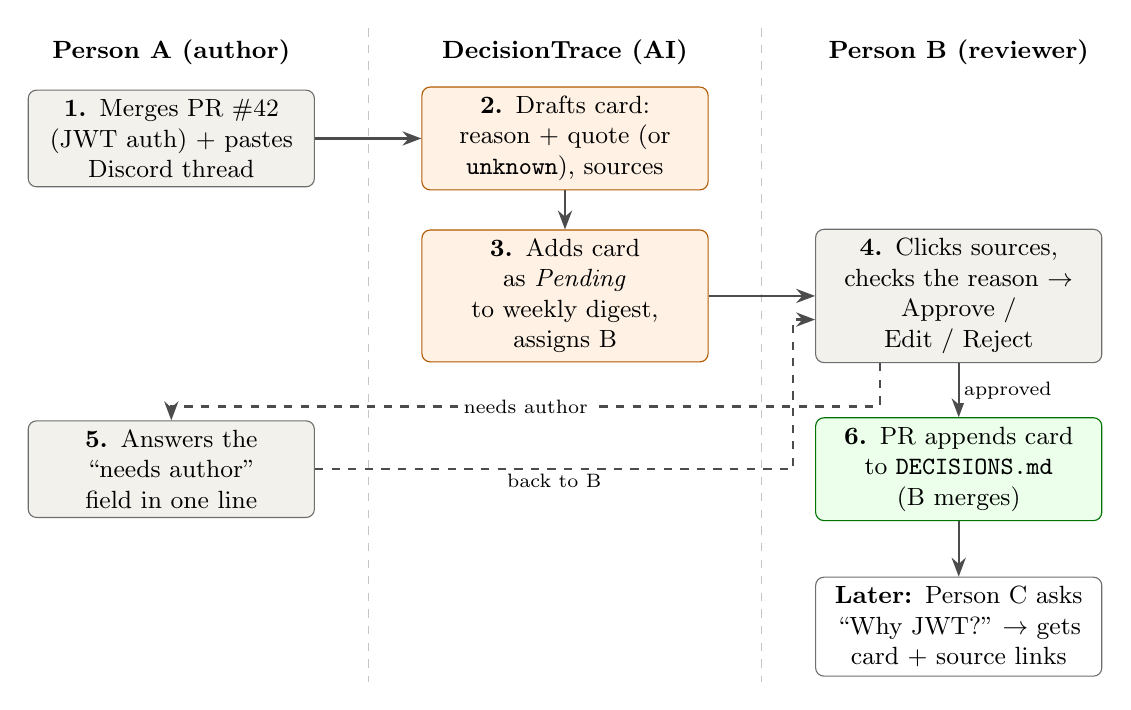
\begin{tikzpicture}[
  box/.style={draw=codecm,rounded corners=3pt,fill=codebg,align=center,font=\small,minimum height=1.15cm,text width=3.4cm},
  ai/.style={box,fill=orange!10,draw=orange!70!black},
  log/.style={box,fill=green!8,draw=green!45!black},
  lane/.style={font=\bfseries\small,text=black},
  arr/.style={-{Stealth[length=2.4mm]},thick,draw=black!70},
  lbl/.style={font=\scriptsize,fill=white,inner sep=1.5pt}
]
\node[lane] at (0,1.1)  {Person A (author)};
\node[lane] at (5,1.1)  {DecisionTrace (AI)};
\node[lane] at (10,1.1) {Person B (reviewer)};
\draw[codecm!40,dashed] (2.5,1.4) -- (2.5,-6.9);
\draw[codecm!40,dashed] (7.5,1.4) -- (7.5,-6.9);

\node[box] (a1)  at (0,0)    {\textbf{1.} Merges PR \#42\\(JWT auth) + pastes\\Discord thread};
\node[ai]  (ai2) at (5,0)    {\textbf{2.} Drafts card:\\reason + quote (or\\\code{unknown}), sources};
\node[ai]  (ai3) at (5,-2)   {\textbf{3.} Adds card as \emph{Pending}\\to weekly digest,\\assigns B};
\node[box] (b4)  at (10,-2)  {\textbf{4.} Clicks sources,\\checks the reason \ra\\Approve / Edit / Reject};
\node[box] (a5)  at (0,-4.2) {\textbf{5.} Answers the\\``needs author''\\field in one line};
\node[log] (l6)  at (10,-4.2){\textbf{6.} PR appends card\\to \code{DECISIONS.md}\\(B merges)};
\node[box,fill=white] (c7) at (10,-6.2) {\textbf{Later:} Person C asks\\``Why JWT?'' \ra{} gets\\card + source links};

\draw[arr] (a1) -- (ai2);
\draw[arr] (ai2) -- (ai3);
\draw[arr] (ai3) -- (b4);
\draw[arr] (b4) -- node[lbl,right]{approved} (l6);
\draw[arr] (l6) -- (c7);
\draw[arr,dashed] ([xshift=-1.0cm]b4.south) -- ++(0,-0.55) -| node[lbl,pos=0.25]{needs author} (a5.north);
\draw[arr,dashed] (a5.east) -- node[lbl,below]{back to B} (7.9,-4.2) |- ([yshift=-0.3cm]b4.west);
\end{tikzpicture}
\end{center}

\textbf{Hand-off summary:} A \ra{} AI \ra{} B (\ra{} A if there is a gap) \ra{} log \ra{} C. A supplies context, the AI only drafts, and B is the gatekeeper who checks the card against its sources. The author never approves their own card.

\subsection{Missing evidence, reversed decisions, and unsupported reasons}

\begin{itemize}
  \item \textbf{Missing evidence.} If the sources do not state a reason, the field is \code{unknown}. B may approve the card as it is (``we chose JWT; reason not recorded'' is still useful) or mark it ``needs author''. If A cannot remember either, it stays \code{unknown}. The AI never fills the gap. A reason supplied by A later is labelled \code{recalled by author (name, date)}, kept separate from \code{stated in source}, and counted separately in the audit (\S\ref{sec:threshold}), because authors can misremember (R1's author was unsure of the reason).
  \item \textbf{Reversed decisions.} When drafting, the AI also sees the titles of already-approved cards and may flag ``possibly supersedes card \#N''. Only B can confirm it. The old card is then marked \code{superseded by \#M} and stays in the log; a question returns the newest card together with the chain of earlier ones. Any teammate can also mark a card superseded by hand.
  \item \textbf{Unsupported reasons.} Four layers: (1) the prompt allows only reasons stated in the sources; (2) a deterministic check (plain string matching, no AI) rejects any reason whose quoted passage does not appear verbatim in the ingested sources, and sets it to \code{unknown}; (3) B confirms that the quote actually supports the reason, which the string check cannot judge; (4) questions are answered only from approved cards. The string check only shows that a quote exists in the text that was ingested, not that the pasted text is complete or authentic; \S\ref{sec:threshold} audits whether these layers are enough.
\end{itemize}

\subsection{v1 scope}\label{sec:scope}

{\small
\begin{tabularx}{\linewidth}{@{}>{\bfseries\raggedright\arraybackslash}p{2.8cm}L@{}}
\toprule
v1 (weeks 8--10) & GitHub REST ingestion for one repository; pasted chat text and Markdown notes; card drafting through an LLM API; the verbatim-quote check; a small web review page with Approve / Edit / Reject / needs author; a weekly digest link posted to Discord by webhook; an auto-opened PR to \code{DECISIONS.md}; questions answered by searching approved cards.\\
Later (only if the evaluation supports it) & Discord bot ingestion; Approve buttons inside Discord (R1) or inside GitHub PR review; LINE export; automatic detection of reversed decisions.\\
\bottomrule
\end{tabularx}
}

\textbf{Design choices informed by interviews [R1, R2], still hypotheses [H]} (to be checked with additional participants):
\begin{itemize}
  \item \textbf{Batched review, not constant notifications} (R2): pending cards are collected into one weekly review digest, whose link is posted in Discord before the weekly sync ($\sim$15 min budget). Each card has one-click Approve / Edit / Reject on the review page (R1).
  \item \textbf{Rotating reviewer} (R2 would reject the tool if they again ended up the only reviewer): cards are assigned round-robin to someone other than the author.
  \item \textbf{Few, non-trivial cards} (R1, R2): the AI must skip routine PRs. The target is $\leq$\,5 cards per week for a 4-person team (R1 would approve 3--5 a week; R2 would reject $\sim$30 trivial ones).
  \item \textbf{\code{reason: unknown} instead of a guess} (R1, R2), plus exact source links on every claim (R1).
  \item \textbf{Statuses beyond approve:} \code{temporary / revisit} (R1) and \code{superseded by \#\ldots} mark decisions that were later reversed.
  \item \textbf{Privacy and consent} (R1): the team agrees in advance which channels or threads are opted in, and nothing from other channels is ingested. The author removes off-topic messages before pasting. Following \code{AI\_GUIDELINES.md}, no credentials or personal data are sent to the LLM API.
\end{itemize}

\textbf{Open design questions:}
\begin{itemize}
  \item Whether pasting chat text is acceptable. A Discord bot needs server permissions and v1 has no LINE integration, so v1 relies on pasted text. This conflicts with R2, who would reject a tool that needed a manual LINE export every time, so we treat the author's preparation time as an adoption risk and measure it (\S\ref{sec:eval}).
  \item Whether a separate review page will be ignored. R1 said a separate site would be ignored; v1 still uses one, because buttons inside Discord need a bot. We will watch whether digests go unreviewed.
\end{itemize}

%==========================================================
\section{Draft Evaluation Plan}\label{sec:eval}
%==========================================================

\subsection{Success definition}\label{sec:success}

\begin{keybox}
\textbf{We will know DecisionTrace works if} students who did \emph{not} take part in a project can answer ``why did the team choose X?'' questions about it \textbf{at least 30\% faster (median time) than students searching the raw GitHub and chat history, with equal or better accuracy ($\geq$\,80\% correct against our ground truth)}, and if \textbf{reviewers accept (approve or edit) at least 60\% of AI-drafted cards while spending a median of $\leq$\,2 minutes per card}.
\end{keybox}

The first half measures the benefit for people who need the reasoning; the second, whether the human review step is affordable for the ``team memory'' person (R2: $\sim$15 minutes a week). The retrieval comparison shows whether an approved log helps at all; any well-kept hand-written log might do as well. The claim specific to DecisionTrace, that AI drafting makes such a log cheap enough to keep, rests on the review-cost criterion and the preparation-time measures.

\textbf{Why these thresholds.} The 2-minute median is deliberately conservative: R2's $\sim$15 min/week budget over at most 5 cards a week (R1's 3--5) would allow 3 minutes per card even if one person reviewed every card, and rotation spreads the cards across three non-authors. The 30\% speed-up is our judgment of the smallest gain that would justify the review cost; it does not come from the interviews and will be revisited after the pilot. These figures come from two interviews [R1, R2] and our own judgment. We will check them with additional participants in weeks 8--9 and record any change to a threshold, with its reason, in \code{DECISIONS.md} before the formative evaluation starts.

\subsection{Target users and how we will reach them}
\begin{itemize}
  \item \textbf{Who:} at least \textbf{6 NYCU students outside our team} (we aim for 8) who have done at least one multi-week team software project, e.g.\ students from other groups in this course or CS students in other project courses.
  \item \textbf{How we will reach them:} (1) ask other groups in this course during or after class and through the course Discord/E3 forum; (2) each team member recruits 2 people from their own lab or department contacts; (3) offer a small incentive (drinks) for a $\sim$25-minute session. Anyone who has seen our test artifacts is excluded.
  \item \textbf{Reviewer role:} 2--3 \emph{additional} participants who have been team leads or maintainers act as card reviewers. They do not take the retrieval task, because reviewing the cards reveals the answers.
  \item \textbf{Totals:} each run needs 6--8 retrieval participants plus 2--3 reviewers; interviewees and anyone who took part in an earlier run are not reused. Because most are recruited through our own contacts, ratings are diagnostic only (politeness bias).
\end{itemize}

\subsection{Method and timing}\label{sec:method}

\textbf{Method: structured observation} (timed tasks with a fixed protocol), followed by a short post-task rating (confidence 1--5, usefulness 1--5).
\begin{itemize}
  \item \textbf{Artifact set.} One fixed history from a real past student project (PRs, issues, commits, a chat export and meeting notes), anonymized before any LLM processing and used with the permission of all its members. We will ask the members of a past course project in our network and aim to have every member's consent by the end of week 9. If that fails, we fall back to a short synthetic project history written by another course group, which none of our participants has seen.
  \item \textbf{Ground truth.} Before DecisionTrace is run on the set, two team members independently list its significant decisions and the reasons the sources state (with quotes). A third member resolves disagreements. Decisions whose reason was never recorded are kept as ``not recorded''. The list and the 3 retrieval questions are committed to the repository before any card is drafted, so neither can be tuned to the tool's output.
  \item \textbf{Review task (runs first):} each AI-drafted card is assigned to one reviewer participant (round-robin). We record approve/edit/reject and time for each card. The cards approved by the assigned reviewer form the log used in the retrieval task, so reviewer mistakes carry through to the result rather than being hidden by a log curated by our team. Outside reviewers lack the context a real teammate has, so this task measures whether a card can be checked against its sources, not full team review. If fewer than 10 cards are drafted, we report acceptance as counts, not a percentage.
  \item \textbf{Retrieval task:} participants are randomly assigned to a \emph{manual} group (raw GitHub + chat export) or a \emph{DecisionTrace} group (approved decision log). Both groups answer the \textbf{same 3 ``why'' questions}: one is answerable from a PR, one needs the chat export, and one has a reason that was never recorded (correct answer: ``not recorded''). Participants in both groups may answer ``not recorded'' at any time. Each question is capped at 6 minutes; a timeout counts as incorrect, is recorded as 360\,s, and is reported as non-completion. The ``not recorded'' question is reported separately and excluded from the pass/fail criteria. Answers are scored against the ground truth by someone not told the participant's group (partial blinding).
  \item \textbf{Preparation overhead:} a team member times the work of selecting and pasting the chat threads for the artifact set. From week 10 we also use v1 on our own repository and log the author's preparation time and the reviewer's time for each card.
\end{itemize}

{\small
\begin{tabularx}{\linewidth}{@{}>{\raggedright\arraybackslash}p{2.8cm}L@{}}
\toprule
\textbf{Measure type} & \textbf{Measures}\\
\midrule
\textbf{Pass/fail} (\S\ref{sec:threshold}) & Median time per question; accuracy; card acceptance rate; median review time per card; unsupported reasons in approved cards.\\
\textbf{Diagnostic} (reported, not pass/fail) & Detection precision and recall; reviewer missed-error rate (wrong drafts approved unchanged); author preparation time per card; results on the ``not recorded'' question; non-completion rate; confidence and usefulness ratings.\\
\bottomrule
\end{tabularx}
}

A high acceptance rate alone does not show that extraction is correct, because a reviewer may approve a wrong card. We therefore read it together with precision, the missed-error rate and the hard rule on unsupported reasons.

\textbf{Timing (rough):}

{\small
\begin{tabularx}{\linewidth}{@{}>{\bfseries}p{1.6cm}L@{}}
\toprule
Week & Activity\\
\midrule
7 & Two real interviews (R1, R2, \S\ref{sec:evidence}) summarized and submitted with CP1.\\
8--9 & At least 3 additional real interviews (late joiner, maintainer, reviewer); revise \S\ref{sec:problem}--\S\ref{sec:eval} if they disagree. Secure the artifact set and its members' consent (fallback decided at the end of week 9).\\
8--10 & Build v1 (scope in \S\ref{sec:scope}).\\
10--14 & Use v1 on our own repository; log preparation and review time per card.\\
11 & Prepare the artifact set; freeze the ground truth and the 3 questions. Pilot the protocol with 1 person.\\
\rowcolor{codebg} 12--13 & \textbf{Formative evaluation}: reviewer sessions first, then at least 6 retrieval participants.\\
14 & Revise prompts and UI based on the results.\\
15--16 & Final evaluation run for the final report.\\
\bottomrule
\end{tabularx}
}

\subsection{Minimum evidence threshold}\label{sec:threshold}

A skeptic should be convinced only if \textbf{all} of the following hold:
\begin{enumerate}
  \item \textbf{At least 6 participants} complete the retrieval task (at least 3 per condition), and at least 2 reviewer participants complete the review task.
  \item The DecisionTrace group gets \textbf{$\geq$\,80\% of answers correct} on the two scored questions (with 3 participants, at least 5 of 6 answers), with \textbf{no lower accuracy} than the manual group.
  \item On the two scored questions, the DecisionTrace group's \textbf{median time is at least 30\% lower} than the manual group's, \textbf{and} every DecisionTrace participant's own median time is below every manual participant's. Each participant's time is the median over their scored questions, with timeouts counted as 360\,s.
  \item Reviewers \textbf{approve or edit at least 60\%} of AI cards, at a \textbf{median of $\leq$\,2 min per card}.
  \item \textbf{No} approved card contains a reason that its cited sources do not support. Two team members independently audit every approved card: each reason must be traceable to a quoted passage in its cited sources that actually states it, and a third member settles disagreements. We report the auditors' agreement, and reasons labelled \code{recalled by author} are counted separately. Even one unsupported ``official'' reason would mean the tool makes the problem worse, so this is a hard failure.
\end{enumerate}

\textbf{Honest limitation:} with 3 per group, individual differences can easily outweigh the tool's effect, which is why item~3 also requires complete separation. If the tool had no effect, every DecisionTrace participant would be faster than every manual participant only about 1 time in 20 with 3 per group (a one-sided permutation test). A smaller or overlapping difference counts as ``not yet shown'', and if the threshold is not met we will report that.

\subsection{Human--AI boundary}

DecisionTrace uses AI (an LLM called through an API).

{\small
\begin{tabularx}{\linewidth}{@{}LL@{}}
\toprule
\textbf{The AI decides / does} & \textbf{The human decides}\\
\midrule
Which passages in the sources \emph{look like} a decision; drafts a candidate card. & Whether it is a real team decision at all (approve vs.\ reject).\\
Wording of decision, reason and alternatives, \textbf{only from what the sources state}, with a quote for each reason; marks a field \code{unknown} otherwise. & Whether the reason is correct and complete (edit), including asking the author.\\
Which source links support each field, and a confidence level. & Whether the card becomes official. \textbf{Nothing enters \code{DECISIONS.md} without a recorded human approval.}\\
Whether a new card may supersede an approved one (a flag only). & Whether it actually does; only the reviewer can mark a card superseded.\\
Which approved card best matches a later question. & Whether to trust the answer; the user can open every source link.\\
\bottomrule
\end{tabularx}
}

The verbatim-quote check is ordinary code, not AI. The AI never publishes, never merges, and never presents an inferred reason as fact. The author of a change cannot approve the card about their own change.

%==========================================================
\section{Repository}\label{sec:repo}
%==========================================================

\textbf{Link:} \url{https://github.com/Apollo58168/NYCU_AI-in-the-Loop-in-Software-Project-Cycle}

{\small
\begin{tabularx}{\linewidth}{@{}>{\raggedright\arraybackslash}p{4.2cm}L@{}}
\toprule
\textbf{Requirement} & \textbf{Status}\\
\midrule
Branch protection on \code{main} & Enabled through the active repository ruleset \href{https://github.com/Apollo58168/NYCU_AI-in-the-Loop-in-Software-Project-Cycle/rules/23748401}{\code{main}} (created 2026-09-21): merging requires a pull request with at least \textbf{1 approving review}, and force-pushes and branch deletion are blocked. The ruleset page is publicly visible. The initial setup commits (repository creation, PR template, \code{DECISIONS.md}) were pushed directly on 2026-09-21 while the ruleset was being configured. Every change since then has gone through a PR (\#1, \#3--\#6 merged; \#2 closed without merging).\\
PR template & \href{https://github.com/Apollo58168/NYCU_AI-in-the-Loop-in-Software-Project-Cycle/blob/main/.github/PULL_REQUEST_TEMPLATE.md}{\code{.github/PULL\_REQUEST\_TEMPLATE.md}}\\
\code{DECISIONS.md} started & \href{https://github.com/Apollo58168/NYCU_AI-in-the-Loop-in-Software-Project-Cycle/blob/main/DECISIONS.md}{\code{DECISIONS.md}}, entry \emph{2026-09-21 --- Initial code steward}\\
Current code steward & \textbf{林彥宇} (\href{https://github.com/Apollo58168}{@Apollo58168}), recorded in the \code{DECISIONS.md} entry \emph{2026-09-21 --- Initial code steward} (unchanged since)\\
\bottomrule
\end{tabularx}
}

Supporting documents already in the repo:\newline \href{https://github.com/Apollo58168/NYCU_AI-in-the-Loop-in-Software-Project-Cycle/blob/main/AI_GUIDELINES.md}{\code{AI\_GUIDELINES.md}}, \href{https://github.com/Apollo58168/NYCU_AI-in-the-Loop-in-Software-Project-Cycle/blob/main/EVALUATION_PLAN.md}{\code{EVALUATION\_PLAN.md}} (the Week~3 version; \S\ref{sec:eval} of this report supersedes it), \href{https://github.com/Apollo58168/NYCU_AI-in-the-Loop-in-Software-Project-Cycle/blob/main/PROMPT_LOG.md}{\code{PROMPT\_LOG.md}}, \code{CONTRIBUTORS.md}.


%==========================================================
\appendix
\section*{Appendix A --- Interview guide}

Guide used for R1 and R2. \emph{Before starting:} explain the project in one sentence, ask whether we may take notes and quote them anonymously, and confirm they are not a member of our team.

\begin{enumerate}
  \item Tell me about the last time you needed to know why your team made an earlier technical decision.
  \item Where did you look, in what order, how long did it take, and did you find the answer?
  \item Did you ask a teammate? How did that go?
  \item Did your team keep a decision log, ADR or meeting notes? Was it maintained? Why or why not?
  \item What went wrong because the reasoning was hard to find?
  \item What specifically do your current tools (chat search, GitHub, notes) fail to do here?
  \item If a tool drafted decision cards that a teammate must approve, what would make you trust it or not? Would you review them?
  \item Anything else?
\end{enumerate}

\end{document}
